\begin{center}
{\textbf{Mardi 24 août : La fin des entraînements !}}
\end{center}
\vspace{2mm}

C’est un réveil matinal qui attend le groupe D. Pour ces élèves, l'entrainement dure 4h et commence donc plus tôt entraînement de 4h. Alors que ces derniers composent déjà, les autres groupes émergent peu à peu et se mettent à leur tour en place dans leurs salles respectives, armés de stylos et feuilles, prêts à affronter l’entraînement de fin de stage.

À 12h, les élèves sortent enfin tous, échangeant avec entrain les idées qu’ils ont pu avoir pendant qu’ils se dirigent vers la cantine. Plusieurs activités organisées par les animatheurs sont proposées aux élèves, avec en jeu phare : Martin-Théo-Géo ! Chaque élève a des papiers Martin, Théo, Géo, et chaque fois qu’il rencontre un élève du groupe ennemi, il peut provoquer un duel. Chacun va brandir un papier en même temps, et la victoire est décidée de cette manière : Martin gagne contre la géo, la géo contre Théo et Théo contre Martin. Le gagnant récupère le papier de l’autre. Si les deux élèves ont utilisé le même papier, c’est match nul et chacun repart de son côté. De plus, les animatheurs ont rajouté des cartes spéciales… Les règles étant un peu compliquées, le jeu a rapidement viré en poule-renard-vipère, plus classique.

\begin{figure}[H]
\centering\includegraphics[width=6cm]{CR-24-0.jpg}\hspace{2cm}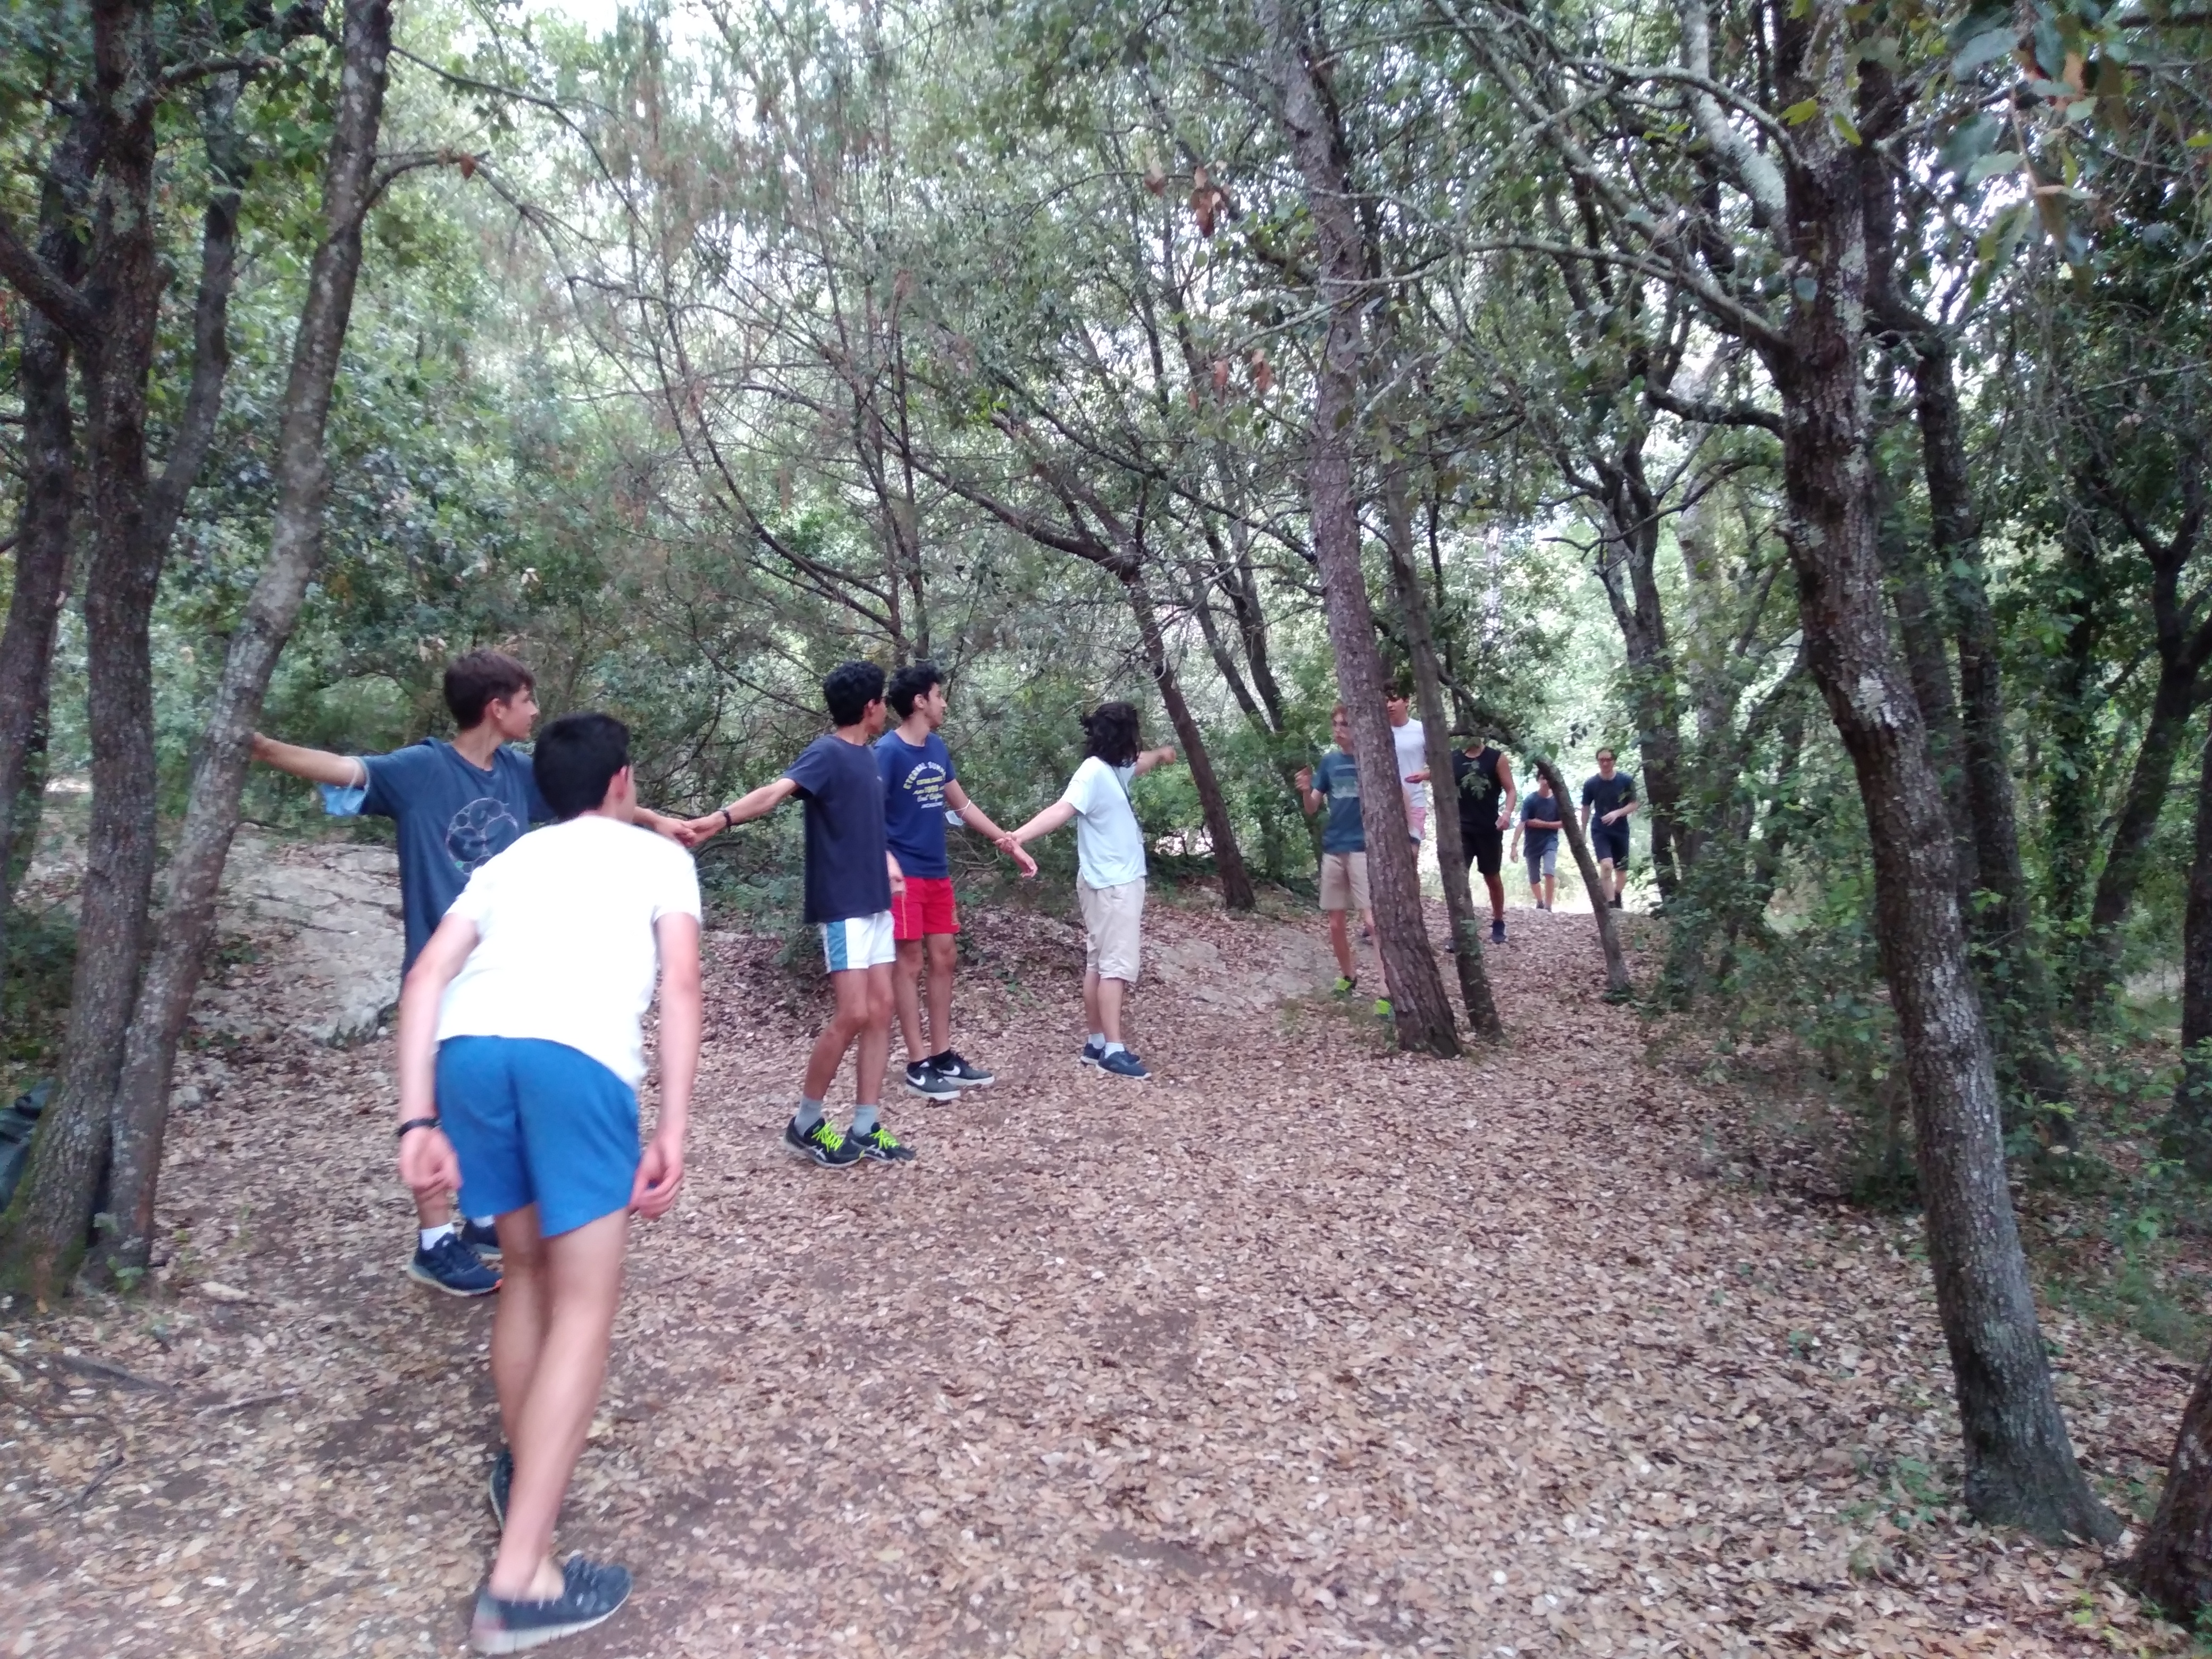
\includegraphics[width=6cm]{CR-24-1.jpg}
\caption{Martin ? Théo ? Géo ! Qui sera le plus fort de la poule, du renard et de la vipère ?}
\end{figure}

Certains élèves ont préféré une activité plus calme et ont opté pour une après-midi jeu de société. Devant l’amphithéâtre de l’autre côté du CIV, ceux-ci ont passé plusieurs heures à jouer aux nombreux jeux proposés par Benoît et Savinien, avant d’être interrompus par l’arrivée du goûter et des sportifs attirés par celui-ci.

\begin{figure}[H]
\centering\includegraphics[height=7cm]{CR-24-2.jpg}\hspace{2cm}\includegraphics[height=7cm]{CR-24-3.jpg}
\caption{Concentration pour les adeptes de jeux ! ? L'heure du goûter !}
\end{figure}

La journée se termine par la correction des entraînements et la remise des copies tant attendue par les élèves. Chaque correcteur passe dans les groupes pour faire un compte-rendu du problème qu’il a corrigé et les élèves peuvent ensuite vaquer à leurs occupations jusqu’à l’heure du couvre-feu.

\begin{figure}[H]
\centering\includegraphics[width=6cm]{CR-24-4.jpg}\hspace{2cm}\includegraphics[width=6cm]{CR-24-5.jpg}
\caption{Discriminant s'est invité à la correction des entrainements des groupes A et B.}
\end{figure}